\documentclass[conference]{IEEEtran}
\IEEEoverridecommandlockouts
% The preceding line is only needed to identify funding in the first footnote. If that is unneeded, please comment it out.
\usepackage{cite}
\usepackage{amsmath,amssymb,amsfonts}
\usepackage{algorithmic}
\usepackage{graphicx}
\usepackage{textcomp}
\usepackage{xcolor}
\usepackage{color}
\usepackage{hyperref}
\def\BibTeX{{\rm B\kern-.05em{\sc i\kern-.025em b}\kern-.08em
    T\kern-.1667em\lower.7ex\hbox{E}\kern-.125emX}}
\begin{document}

\title{Détection des points-clés et calcul des descripteurs dans une image}

\author{
    \IEEEauthorblockN{NAOUSSI SIJOU, Wilfried Armand}
    \IEEEauthorblockA{
        \textit{Département d'informatique} \\
        \textit{Université Laval}, Québec QC, Canada \\
        wilfried-armand.naoussi-sijou.1@ulaval.ca
    }
}

\maketitle

\begin{abstract}
La vision est la perception du monde extérieur à travers des images. En robotique mobile, il s'agit d'extraire des caractéristiques visuelles à partir d'algorithmes qui se basent sur des points d'intérêt dans l'image pour la détection des objets, la localisation, la fermeture de boucle SLAM, etc. On teste dans cette article trois modèles: SIFT et ORB qui sont des méthodes dites faites à la main ainsi que vgg16, un réseau de neurones convolutif, un des gagnants de la compétition de ImageNet en 2014. Nous mettons ainsi en évidence deux critères importants pour les features et l'impact des différents paramètres sur ces derniers. 
\end{abstract}

\begin{IEEEkeywords}
Points-clés, coins, descripteurs, caractéristiques, SIFT, ORB, VGG, CNN
\end{IEEEkeywords}

\section*{Introduction}
La vision est la perception du monde extérieur à travers des images. En robotique mobile, il s'agit de donner la possibilité au robot d'extraire des informations à partir d'une images ou un ensemble d'images (pack d'images, vidéos, etc.) à des fins de classification, détection objets, visages ou personnes, localisation, fermeture de boucle SLAM, etc. Les chercheurs de plus en plus intéressés 
par ce domaine ont trouvé différentes méthodes pour extraire et analyser ces informations. D'une part nous avons les caractéristiques globales que sont les couleurs, la forme et la texture et d'autre part nous avons les caractéristiques locales qui consiste à détecter des zones d'intérêts et d'y extraire un vecteur représentatif. Le présent document porte uniquement sur ce deuxième aspect. \\

Beaucoup de travaux à nos jours ont déjà été réalisés. Tout d'abord le filtre de sobel \cite{b5} qui permet la détection des contours dans une image en calculant le gradient de l'intensité de chaque pixel. Les recherches de Moravec et par la suite de Harris et Stephens ont poussé à la mise au point des algorithmes de détection de coins \cite{b6}. Ceux ci permettent d'obtenir de meilleurs résultats que Sobel et en prime restent très simple à comprendre et à implémenter. Les chercheurs ne s'arrêtent pas là car il s'avère que ces méthodes développer sont sensibles au changement de taille. En réponse de cela, David G. Lowe publie un article \cite{b1} sur une nouvelle méthode qu'il nomme SIFT pour Scale-Invariant Feature Transform. Cette dernière utilise plusieurs transformation de la taille de l'image pour détecter les coins et calculer les descripteurs. Bien sûr plusieurs variations de cet algorithme ont été mise en place. Parmi lesquelles la plus connus est SURF qui se veut plus rapide et plus performante que sont prédécesseur SIFT. ORB \cite{b2} quant à lui a été mise en place quelques années plus tard comme alternative à SIFT et à SURF. Un an plus tard, en 2012, ImageNet organise une compétition où des équipes de recherche évaluent leurs algorithmes de traitement d'images sur le jeu de données ImageNet (un jeu de validation non accessible), et concourent pour obtenir la meilleure précision sur plusieurs tâches de vision par ordinateur \cite{b7}. Le grand gagnant de cette année se trouve être AlexNet un réseau de neurones convolutif. L'apprentissage profond qui avait perdu l'intérêt des scientifiques devient alors de plus en plus sujets dans les discussions. Les années qui suivirent, remporta à leur tour ZFNet, GoogleNet et vgg, resnet, etc.\\

Dans la suite, nous attarderons sur trois méthodes: SIFT, ORB et vgg16. L'objectif de cette étude est de tester les différents algorithmes mentionnés et de voir leur comportement en fonction des différents paramètres pour SIFT et ORB. En ce qui concerne vgg16, nous réaliserons un transfert d'apprentissage sur le réseau préentrainé pour obtenir un vecteur représentatif. Pour cela, nous devons faire deux opérants avant et après. La première consiste à redimensionner le patch d'image extraite pour qu'il puisse fonctionner correctement avec vgg. La seconde, consiste en une opération de compression grâce à un autoencodeur. Ce dernier permet d'obtenir un vecteur de 128 ou 256 qui est plus pratique pour des raisons de rapiditité computationnelle.  

Pour cela, nous utilison le jeu d'images stereos disponible sur le site \href{https://drivingstereo-dataset.github.io/}{DrivingStereo}. Ils fournissent un jeu de données d'images stéreos séparées en deux pack: les images de gauche et les images de droite. Les paires portent le même nom ce qui facilite la correspondance. De plus, les images sont prises de manière succinte d'un déplacement du mobilé à l'autre.

\section{Méthodologie et expérimentation}\label{Method}

SIFT (Scale-Invariant Feature Transform) a été proposé par David G. Lowe en 2004 \cite{b1}, c'est une des méthodes les plus populaires utilisées pour le calcul des descripteurs. 

Dans cette article, nous utilisons l'implémentation offerte par opencv-python via la fonction SIFT\_create(). Parmi ses paramètres, nous faisons varier nOctaveLayers et sigma qui représentent respectivement le nombre de couches dans chaque octave ainsi que la variance de la gaussienne utilisée. \\

La 2ème méthode expérimentée est ORB (Oriented fast and Rotated BRIEF) proposée par Rublee et al en 2011 \cite{b2}. C'est une alternative développée pour remplacer SIFT et SURF. 

A linstar de SIFT, nous utilisons l'implémentation de opencv-python ORB\_create. Opencv utilise par défaut la détection de coins Harris au lieu de FAST comme décris dans \cite{b2}. Mais ceci est modifiable via le paramètres scoreType. Nous faisons varier WTA\_K qui est Le nombre de points qui produisent chaque élément du descripteur BRIEF orienté. Ses seules valeurs possibles sont 2,3 et 4. \\

La dernière méthode quant à elle est le réseau de neurones convolutif vgg16, grand gagnant de la compétition ILSVRC organisée par ImageNet en 2014 \cite{b3}. 

Nous utilisons le modèle préentrainé de pytorch du torchvision.models.vgg16. Tout d'abord, nous utilisons FAST pour détecter les points-clés dans l'image. Puis nous extrayons des patchs d'images de 64x64 autour de chacun de ces points. Nous les passons ensuite à notre réseau qu'on a préalement modifié pour extraire les caractéristiques visuelles. Nous compressons ensuite le vecteur de sortie grâce à un autoencodeur comme décrit dans \cite{b4}. \\

\section{Figures et Résultats}

\subsection{SIFT}

Les figures ci-dessous montrent respectivement le nombre de points-clés trouvés ainsi que le ration nombre de correspondances sur nombre de points-clés pour les différentes méthodes mentionées en \ref{Method}. 

\begin{figure}[ht]
\centerline{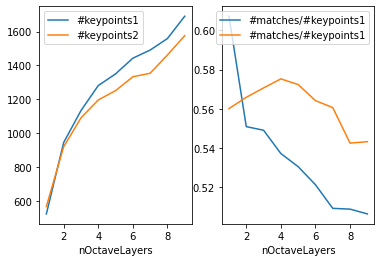
\includegraphics[width=0.5\textwidth]{fig1.png}}
\caption{SIFT nombre de points-clés et ratio correspondances en fonction de nOctaveLayers.}
\label{fig}
\end{figure}

Dans la figure 1 ci-dessus, on observe sur la première courbe que le nombre de points détectés augmentent en fonction du nombre de couches utilisé pour chaque octave. Tandis que la 2ème montre une décroissance du ratio obtenu.

\begin{figure}[ht]
\centerline{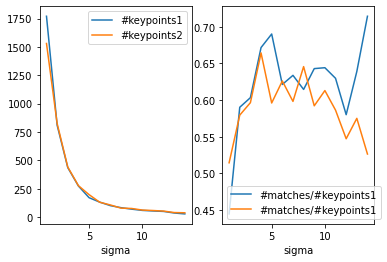
\includegraphics[width=0.5\textwidth]{fig2.png}}
\caption{SIFT nombre de points-clés et ratio correspondances en fonction de sigma.}
\label{fig}
\end{figure}

Dans la figure 2, la première courbe montre une décroissance du nombre de points-clés au fur et à mesure que sigma augmente.  La figure 2 par contre montre une forme d'escaliers qui montent et descend. \\

\subsection{ORB}

\begin{figure}[ht]
\centerline{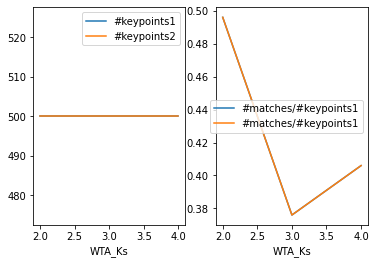
\includegraphics[width=0.5\textwidth]{fig3.png}}
\caption{ORB nombre de points-clés et ratio correspondances en fonction de WTA\_K.}
\label{fig}
\end{figure}

Dans la figure 3, On voit qu'on a un nombre constant de points-clés pour les différentes valeurs possibles de WTA\_K. La deuxième courbe par contre montre une chute du ratioi qui passe d'environ 0.50 à 0.38 puis remonte à 0.41. \\

\subsection{VGG16}
Dans le cas, de la dernière méthode, nous n'avons pas aboutit à un résultat concluant. D'où le manque de figure.

\section{Discussion}

L'hypothèse émise derrière ces expériences étaient de mettre en évidence la répétitivité et la distinctivité des points-clés générés par les différents algorithmes. 

Pour la première mesure, je compare le nombre de points-clés obtenus dans chaque image. Dans notre cas, ce sont des images stéréos (gauche, droite). Nous avons donc des images, quasi-identiques. Ceci implique qu'on devrait obtenir un nombre égale de points-clés dans chacune des images (ou presque). 

Pour la seconde, nous avons déterminé à l'instar du ratio de compétitivité,  un ratio qui s'en rapproche. Le but étant de comparer nos algorithmes avec un algorithme dit optimal. Plus il est grand, plus on considèrera que nos vecteurs sont différentiables.

Ainsi, on voit que plus nOctaveLayers est grand plus le nombre de points-clés trouvés devient différent dans nos images de gauche et de droite. Inversément, cela décroit notre ratio. 

Les résultats obtenus pour la courbe s'explique par le fait que WTA\_K est pris en compte uniquement après que les points-clés aient été détectés. Donc ce paramètre n'influence pas le nombre de points-clés obtenus. 
La deuxième courbe quant à elle, montre qu'on obtient les meilleurs performance en terme de correspondance avec WTA\_K=2.

Dans, le cas de vgg16, nous n'avons pas pu le faire fonctionner correctement. 

Ceci s'explique par le fait que nous ne possédons pas une machine assez puissance pour faire beaucoup de test. 

Chaque exécution met un temps considérable avant d'afficher le résultat. Ce qui constitue également un gros problème dans le cadre de la robotique mobile.

\section*{Conclusion}

Les travaux réalisés dans cet article avaient pour but de voir le comportement des algorithmes SIFT, ORB en fonction de leurs différents paramètres. Il a été mis en évidence ici deux des critères clés d'une bonne caractérisitique. Par contre, pour la robustesse, nous n'avions aucune référence dans notre jeu de données pour la mesurer. Nous aurions pu par contre, estimer la distance entre notre mobile et les différents points appariés ou encore l'utiliser pour la fermeture de boucle SLAM.

\begin{thebibliography}{00}
\bibitem{b1} David G. Lowe, 'Distinctive Image Features from Scale-Invariant Keypoints', 05 Janvier 2004.
\bibitem{b2}  Rublee, Ethan; Rabaud, Vincent; Konolige, Kurt; Bradski, Gary, 'ORB: an efficient alternative to SIFT or SURF', 2011.
\bibitem{b3} NeuroHive, 'VGG16 – Convolutional Network for Classification and Detection', 20 November 2018
\bibitem{b4} Zhuang Dai et al., 'A Comparison of CNN-Based and Hand-Crafted Keypoint Descriptors', 2021
\bibitem{b5} Wikipédia, 'Filtre de Sobel'
\bibitem{b6} Wikipedia, 'Corner detection'
\bibitem{b7} Wikipédia, 'ImageNet'
\end{thebibliography}
\vspace{12pt}
\color{red}

\end{document}
